\documentclass[final,table,svgnames]{article}
\usepackage{graphicx}
\usepackage{tikz}
\usepackage{pgfpages}
\usepackage{xcolor}
\usepackage{subcaption}
\usepackage{hyperref}
\usepackage[margin=0.25in]{geometry}

\hypersetup{bookmarksopen=true,
bookmarksnumbered=true,  
pdffitwindow=false, 
pdfstartview=FitH,
pdftoolbar=false,
pdfmenubar=false,
pdfwindowui=true,
pdfauthor=Charles Troupin,
pdftitle=Charles Troupin Curriculum,
pdfsubject=C. Troupin Resume,
colorlinks=true,%
breaklinks=true,%
linkcolor=blue,anchorcolor=blue,%
citecolor=blue,filecolor=blue,%
menucolor=blue,%
urlcolor=blue}

\tikzstyle{na} = [baseline=-.5ex]
\usetikzlibrary{arrows,shapes,backgrounds}
\tikzstyle{every picture}+=[remember picture]
\usetikzlibrary{spy}


\usepackage{fontspec}
\defaultfontfeatures{Ligatures=TeX}
\tikzset{mynode/.style={draw,solid,circle,inner sep=1pt,fill=yellow}}

   
% ------------------------------------------------
% LENGTH DEFINITIONS
%-------------------------------------------------
%\setlength{\textwidth}{24cm}
%\setlength{\textheight}{28cm}

\DeclareGraphicsExtensions{.eps,.JPG,.jpg,.pdf,.png,.PNG,.jpeg}
\graphicspath{../figures/}

% These lines to keep good colors when viewed with Acrobat Reader
\makeatletter%
\special{pdf: put @thispage <</Group << /S /Transparency /I true /CS /DeviceRGB>> >>}%
\makeatother%

\begin{document}
\pagestyle{empty}

\begin{figure}

\begin{subfigure}[t]{.35\textwidth}
\caption{Ocean color image using data collected during two orbits of the Suomi-NPP/VIIRS instrument on December 10, 2018. Source: OceanColor \url{https://oceancolor.gsfc.nasa.gov/}}
\includegraphics[width=\textwidth]{../figures/V2018344.CanaryUpwelling_cropped.jpg}
\end{subfigure}\hspace{1cm}
\begin{subfigure}[t]{.4\textwidth}
\caption{Temporal and spatial scales of oceanic processes.}
\includegraphics[width=\textwidth]{../figures/oceanscales.png}
\end{subfigure}

\begin{subfigure}[b]{.85\textwidth}
\caption{Sea surface temperature for the summer 2018. Black arrows depict wind in the four Eastern Boundary Current Upwelling Systems (EBUS). The large arrows show the mean wind vector averaged over the upwelling areas.}
\includegraphics[width=.85\textwidth]{../figures/SST_wind_summer_2018_08.png}
\end{subfigure}

\begin{subfigure}[b]{.8\textwidth}
\caption{Sea surface temperature corresponding to September 4, 2017. An upwelling filament is enlarged inside the circle. Data from VIIRS on board Suomi-NPP.}
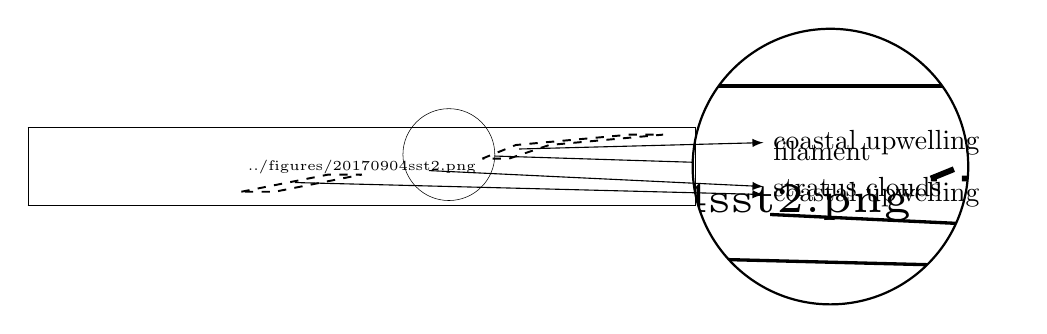
\begin{tikzpicture}[spy using outlines={circle,black,magnification=3,size=3.5cm, connect spies}]
\node[anchor=south west,inner sep=0] (image) at (0,0) {\pgfimage[interpolate=true,width=.7\textwidth]{../figures/20170904sst2.png}};
   
    \begin{scope}[x={(image.south east)},y={(image.north west)}]
%    \draw[help lines,xstep=.1,ystep=.1] (0,0) grid (1.1,1.1);
%    \foreach \x in {0,1,...,10} { \node [anchor=north] at (\x/10,0) {\x}; }
%    \foreach \y in {0,1,...,10} { \node [anchor=east] at (0,\y/10) {\y}; }
    \coordinate (center) at (0.63,0.65);
    \coordinate (pos spy) at (1.2,.5);
	\spy on (center) in node [] at (pos spy);
  
    \path[draw,line width=.7pt,style=dashed] (0.32,0.185) -- (0.45,0.4)--(0.5,0.4)--(0.37, 0.185)--cycle;
    
    \path[draw,line width=.7pt,style=dashed] (0.68,0.6) -- (0.73,0.77)--(0.9,0.9)--(0.95, 0.90)--(.78, .77)--(.72, .6)--cycle;
    
    \draw[-latex] (0.6, 0.45) -- (1.1,0.25)node[anchor=west,font=\normalsize]{stratus clouds};
    \draw[-latex] (0.4,0.3) -- (1.1,0.15)node[anchor=west,font=\normalsize] {coastal upwelling};
    \draw[-latex] (0.735,.72) -- (1.1, 0.8) node[anchor=west,font=\normalsize] {coastal upwelling};
    \node[text width=3cm,anchor=west,font=\normalsize] at (1.1,.7) {filament};
	
    \end{scope}  
\end{tikzpicture}
\end{subfigure}



\end{figure}



\end{document}
